\documentclass[border=3pt,tikz]{standalone}
\usepackage[utf8]{vietnam}
\usetikzlibrary{calc,angles,intersections,shapes.geometric,arrows,decorations.markings,arrows.meta,patterns.meta,patterns}
\usepackage{tikz-3dplot,pgfplots}
\pgfplotsset{compat=1.15}
\usepgfplotslibrary{polar}
\usepackage{amsmath}
\begin{document}
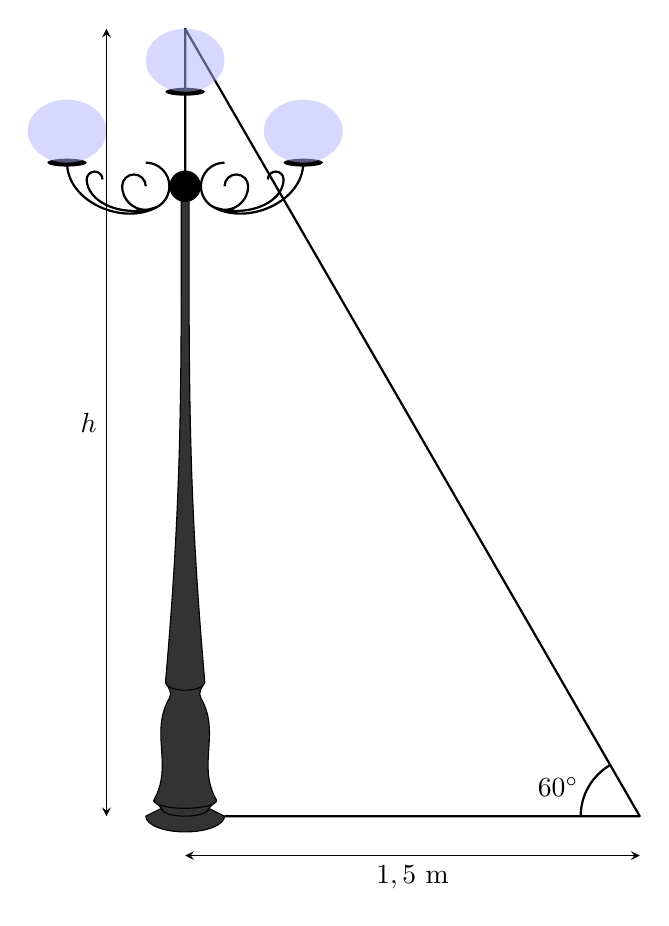
\begin{tikzpicture}[join=round]
	\draw[fill=black!80]
	(-.5,0) arc (180:360:{.5} and {.2})
	--(.3,.1)--(.4,.2)
	to[out=120,in=-60] (.2,1.5)
	to[out=120,in=-120](.25,1.7)
	to[out=95,in=-90] (.05,8)
	--(-.05,8)
	to[out=-90,in=85] (-.25,1.7)
	to[out=-60,in=60] (-.2,1.5)
	to[out=-120,in=60](-.4,.2)
	--(-.3,.1)--cycle
	;
	\fill[black]
	(0,8) circle (.2)
	(0,9.2)ellipse ({.25} and {.05})
	(1.5,8.3)ellipse ({.25} and {.05})
	(-1.5,8.3)ellipse ({.25} and {.05})
	;
	\draw[thick]
	(.5,8.3) arc (90:240:.3) to[out=-30,in=-90] (1.5,8.3)
	(-.5,8.3) arc (90:-60:.3) to[out=-150,in=-90] (-1.5,8.3)
	(.5,8.3) arc (90:240:.3) arc (-120:0:{.6} and {.4}) arc (0:180:.1)
	(-.5,8.3) arc (90:-60:.3) arc (-60:-180:{.6} and {.4}) arc (180:0:.1)
	(.5,8.3) arc (90:360:.3) arc (0:180:.15)
	(-.5,8.3) arc (90:-180:.3) arc (180:0:.15)
	(0,8)--(0,10)--({10/tan(60)},0)--(.5,0)
	({10/tan(60)-.75},0) arc (180:120:.75)node[pos=.5,left]{$60^{\circ}$}
	;
	\fill[blue!30,opacity=.5]
	(1.5,8.7) ellipse ({.5} and {.4})
	(-1.5,8.7) ellipse ({.5} and {.4})
	(0,9.6) ellipse ({.5} and {.4})
	;
	\draw
	(-.3,.1) arc (180:360:{.3} and {.1})
	(-.4,.2) arc (180:360:{.4} and {.1})
	(-.25,1.7) arc (180:360:{.25} and {.1})
	;
	\draw[stealth-stealth] (-1,0)--(-1,10)node[pos=.5,left]{$h$};
	\draw[stealth-stealth] (0,-.5)--({10/tan(60)},-.5)node[pos=.5,below]{$1,5$ m};
\end{tikzpicture}
\end{document}